%----------------------------------------------------------------------------------------
%	PACKAGES AND THEMES
%----------------------------------------------------------------------------------------
\documentclass[aspectratio=169,xcolor=dvipsnames]{beamer}
\usetheme{SimplePlus}

\usepackage{hyperref}
\usepackage{graphicx} % Allows including images
\usepackage{booktabs} % Allows the use of \toprule, \midrule and \bottomrule in tables
\usepackage{tikz}
\usetikzlibrary{shapes.geometric, arrows, shadows, positioning}
\usepackage{tikz-cd}
\usepackage{adforn} % ornaments, used in titlepage

\input xy
\xyoption{all}


% -----------------------------------
% math
% -----------------------------------

\usepackage{amsmath}
\usepackage{amsfonts}
\usepackage{amssymb}
\usepackage{amsthm}
\usepackage{mathrsfs}   % \mathscr
\usepackage{stmaryrd}   % \lightning
\usepackage{mathabx,epsfig}
\usepackage{physics}

% -----------------------------------
% macros
% -----------------------------------

\newcommand{\ra}{\rightarrow}
\newcommand{\la}{\leftarrow}
\newcommand{\lra}{\longrightarrow}
\newcommand{\lla}{\longleftarrow}
\newcommand{\into}{\hookrightarrow}
\newcommand{\Spec}{\operatorname{Spec}}
\newcommand{\Proj}{\operatorname{Proj}}
\newcommand{\NN}{\mathbb{N}}
\newcommand{\ZZ}{\mathbb{Z}}
\newcommand{\QQ}{\mathbb{Q}}
\newcommand{\RR}{\mathbb{R}}
\newcommand{\CC}{\mathbb{C}}
\newcommand{\PP}{\mathbb{P}}
\newcommand{\FF}{\mathbb{F}}
\newcommand{\GG}{\mathbb{G}}
\newcommand{\HH}{\mathbb{H}}
\newcommand{\kk}{\mathbb{k}}
\newcommand{\ee}{\mathbb{e}}
\newcommand{\bbA}{\mathbb{A}}
\newcommand{\TT}{\mathbb{T}}
\newcommand{\half}{\frac{1}{2}}
\newcommand{\Mat}{\text{Mat}}
\newcommand{\Hom}{\operatorname{Hom}}
\newcommand{\Span}{\text{Span}}
\newcommand{\Bl}{\operatorname{Bl}}
\newcommand{\Pic}{\operatorname{Pic}}
\newcommand{\Id}{\operatorname{Id}}
\newcommand{\Td}{\operatorname{Td}}
\newcommand{\Lie}{\operatorname{Lie}}
\newcommand{\mf}[1]{\mathfrak{#1}}
\newcommand{\mfg}{\mathfrak{g}}
\newcommand{\mfk}{\mathfrak{k}}
\newcommand{\mfn}{\mathfrak{n}}
\newcommand{\mft}{\mathfrak{t}}
\newcommand{\mc}[1]{\mathcal{#1}}
\newcommand{\mcL}{\mathcal{L}}
\newcommand{\ed}{e^{\ast}}
\newcommand{\fd}{f^{\ast}}
\newcommand{\semistable}{\text{ss}}
\newcommand{\stable}{\text{s}}
\newcommand{\dual}[1]{#1^{\ast}}
\newcommand{\w}{\omega}
\newcommand{\pt}{\text{pt}}
\newcommand{\GL}{\operatorname{GL}}
\newcommand{\SL}{\operatorname{SL}}
\newcommand{\SU}{\operatorname{SU}}
\newcommand{\Sp}{\operatorname{Sp}}
\newcommand{\PSL}{\operatorname{PSL}}
\newcommand{\Hilb}{\operatorname{Hilb}}
\newcommand{\lat}{\operatorname{lat}}
\newcommand{\gp}{\operatorname{gp}}
\newcommand{\pos}{\operatorname{pos}}
\newcommand{\Diff}{\operatorname{Diff}}
\newcommand{\ind}{\operatorname{ind}}
\newcommand{\td}{\operatorname{td}}
\newcommand{\ch}{\operatorname{ch}}
\newcommand{\coker}{\operatorname{coker}}
\newcommand{\Ver}{\operatorname{Ver}}
\newcommand{\Ad}{\operatorname{Ad}}
\newcommand{\HK}{\operatorname{HK}}
\newcommand{\Image}{\operatorname{image}}

\newcommand{\sssslash}{\mathbin{/\mkern-6mu/\mkern-6mu/\mkern-6mu/}}
\newcommand{\restr}[2]{\left.#1\right|_{#2}}

\def\acts{\mathrel{\reflectbox{$\righttoleftarrow$}}}

%----------------------------------------------------------------------------------------
%	TITLE PAGE
%----------------------------------------------------------------------------------------

\title[short title]{Index Theory for Orbifolds} % The short title appears at the bottom of every slide, the full title is only on the title page
\subtitle{Subtitle}

\author[Pin-Yen] {Pin-Yen Huang}

\institute[NTU] % Your institution as it will appear on the bottom of every slide, may be shorthand to save space
{
    Department of Computer Science and Information Engineering \\
    National Taiwan University % Your institution for the title page
}
\date{\today} % Date, can be changed to a custom date


%----------------------------------------------------------------------------------------
%	PRESENTATION SLIDES
%----------------------------------------------------------------------------------------

\begin{document}

\begin{frame}
    % Print the title page as the first slide
    \titlepage
\end{frame}

\begin{frame}{Overview}
    % Throughout your presentation, if you choose to use \section{} and \subsection{} commands, these will automatically be printed on this slide as an overview of your presentation
    \tableofcontents
\end{frame}

%------------------------------------------------
\section{Orbifolds}
%------------------------------------------------

\begin{frame}{Introduction}
    \begin{itemize}
        \item Orbifolds generalise manifolds in that they locally look like $\RR^{n}/\Gamma$, for $\Gamma$ a finite group.
        \item First introduced by Ichiro Satake in 1956, coining them ``$V$-manifolds''.
        \item After a ``\emph{democratic process}'' in 1976-77, William Thurston recoined them as ``orbifolds''.
        \item Other candidates were ``foldamani'', and ``manifolded''.
    \end{itemize}    
\end{frame}

\begin{frame}{Charts}
	\textcolor{blue}{\underline{Def:}} For $X$ a paracompact Hausdorff space. An \textcolor{red}{orbifold chart} is a triple $(\widetilde{U}, \Gamma, \phi)$:
	\begin{itemize}
		\item $\widetilde{U} \subseteq \RR^{n}$ is open, and $\{0\} \in \widetilde{U}$;
		\item $\Gamma$ finite group, effectively acting on $\widetilde{U}$;
		\item $\phi : \widetilde{U} \ra U$ continuous onto $U \subset X$, \newline such that $\phi \circ \gamma = \phi$, for all $\gamma \in \Gamma$;
		\item Induced $\phi : \widetilde{U}/\Gamma \ra U$ is a homeomorphism.\newline
	\end{itemize}
	
	For two charts, $(\widetilde{U}_{1}, \Gamma_{1}, \phi_{1})$, and $(\widetilde{U}_{2}, \Gamma_{2}, \phi_{2})$: \newline
	
	\textcolor{blue}{\underline{Def:}} An \textcolor{red}{embedding} between them is a smooth embedding $\lambda : \widetilde{U}_{1} \ra \widetilde{U}_{2}$ such that
	\[
	\phi_{2} \circ \lambda = \phi_{1}.    
	\]
\end{frame}

\begin{frame}{Atlases}
	\textcolor{blue}{\underline{Def:}} An \textcolor{red}{orbifold atlas} on $X$ is a family $\mathcal{U} = \{\widetilde{U}_{i}, \Gamma_{i}, \phi_{i}\}$ of charts such that
	\begin{itemize}
		\item $X = \bigcup_{i} \phi_{i}(\widetilde{U}_{i})$;
		\item Two charts $(\widetilde{U}_{1}, \Gamma_{1}, \phi_{1})$, and $(\widetilde{U}_{2}, \Gamma_{2}, \phi_{2})$, with $U_{1} = \phi_{1}(\widetilde{U}_{1})$ and $U_{2} = \phi_{2}(\widetilde{U}_{2})$, and a point $x \in U_{1} \cap U_{3}$, there is an open neighbourhood $U_{3}$ of $x$, and a chart $(\widetilde{U}_{3}, \Gamma_{3}, \phi_{3})$ such that there are embeddings
		\[
		\lambda_{31} : \widetilde{U}_{3} \ra \widetilde{U}_{1}, \quad \lambda_{32} : \widetilde{U}_{3} \ra \widetilde{U}_{2}.
		\]
	\end{itemize}
	\textcolor{blue}{\underline{Note:}} Similarly for manifolds, an orbifold atlas $\mathcal{U}$ has a \textcolor{red}{refinement} $\mathcal{V}$ if each chart $\widetilde{U} \overset{\text{injects}}{\longrightarrow} \widetilde{V}$.
\end{frame}

\begin{frame}{Orbifolds}
    
	\textcolor{blue}{\underline{Def:}} An \textcolor{red}{orbifold} is a paracompact Hausdorff space $X$ with an equivalence class of orbifold atlases.
	\begin{itemize}
		\item Every orbifold has a \emph{unique} maximal orbifold atlas $\mathcal{U}$;
		\item Call the pair $\mathcal{X} = (X, \mathcal{U})$ an orbifold.
	\end{itemize}
\end{frame}

\begin{frame}{Examples}
	\textcolor{blue}{\underline{Examples of orbifolds:}}
	\begin{itemize}
		\item Any manifold $X$ is an orbifold with trivial $\Gamma$.
		\item Let $T^{4} = (\RR/\ZZ)^{4}$, and introduce the $(\ZZ/2\ZZ)$-action:
		\[
		(t_{1}, t_{2}, t_{3}, t_{4}) \mapsto (t_{1}^{-1}, t_{2}^{-1}, t_{3}^{-1}, t_{4}^{-1}).
		\]
		$X := T^{4}/\ZZ_{2}$ quotient is a \textcolor{red}{Kummer surface}, with $|X^{\ZZ_{2}}| = 16$.
	\end{itemize}
    \begin{figure}
        \centering
        \includegraphics[scale=0.075]{Kummer_surface.png}
    \end{figure}
\end{frame}

\begin{frame}{Examples}
	\begin{itemize}
		\item A \textcolor{red}{``mirror''}, i.e. $\RR^{2}/(x \sim -x) \cong \{(x,y) \in \RR^{2}\ |\ x \geq 0\}$.
		\hfill \break
		\item A \textcolor{red}{``barber shop''}, i.e. $\RR^{2}$ quotiented by the relations
		\[
		\{(x \sim -x),\ (1 + x \sim 1 - x)\} \cong (\ZZ/2\ZZ)^{2}.
		\]
		$\rightsquigarrow \RR^{2} / (\ZZ/2\ZZ)^{2} \cong \{(x,y) \in \RR^{2}\ |\ 0 \leq x \leq 1 \}$.
	\end{itemize}
\end{frame}

\begin{frame}{Examples - teardrop orbifold}
	\begin{itemize}
		\item The \textcolor{red}{``teardrop''}.
		
		Let $(z_{1}, z_{2}) \in \CC^{2} - \{0\}$ and $t \in \CC^{\ast}$.
		\[
		t \cdot (z_{1}, z_{2}) = (tz_{1}, t^{p}z_{2}), \quad p \in \NN.
		\]
		Quotient $\left(\CC^{2} - \{0\}\right)/\CC^{\ast}$ topologically is $\CC\PP^{1}$.
		\hfill \break
		\item Fixed-points are $[z_{1}:0]$ and $[0:z_{2}]$.
		\begin{itemize}
			\item $[z_{1}:0]$ is smooth;
			\item $[0:z_{2}]$ is singular, with $\Gamma \cong \ZZ_{p}$.
		\end{itemize}
	\end{itemize}
\end{frame}

\begin{frame}{Examples - toric symplectic orbifolds}
	\textcolor{blue}{\underline{Def:}} A \textcolor{red}{\underline{symplectic toric orbifold}} is a $4$-tuple $(M, \w, T^{n}, \mu)$, such that:
	\begin{itemize}
		\item $(M,\w)$ is a $2n$-dim. connected symplectic orbifold;
		\item $T^{n}$ is an $n$-torus, with an effective and Hamiltonian action on $M$;
		\item $\mu : M \ra \RR^{n}$ is a moment map for the $T^{n}$-action.
	\end{itemize}
	\hfill \\
	\textcolor{blue}{\underline{Thm:}} Symplectic toric orbifolds $(M, \w, T^{n}, \mu)$ are classified by \textcolor{red}{\underline{simple}} convex polytopes $\Delta \subseteq \RR^{n}$, where $\mu(M) = \Delta$ is the convex hull of the fixed-points for the $T^{n}$-action on $M$.
\end{frame}

\begin{frame}{Examples - toric symplectic orbifolds}
	Convex polytope $\Delta \subseteq \RR^{n}$ represented as an intersection of half-spaces;
	\[
		\Delta = \bigcap_{i=1}^{N} \{ y \in \RR^{n}~|~\langle y, u_{i}\rangle + \lambda_{i} \geq 0 \}.
	\]
	\begin{itemize}
		\item The $u_{i} \in (\RR^{n})^{\ast}$ represent the \textcolor{red}{\underline{normal vector}} to the $i$-th hyperplane;
		\item The $\lambda_{i} \in \RR$ determine the half-space locations.
	\end{itemize}

	\begin{figure}[h!]
		\centering
		\scalebox{0.45}{
		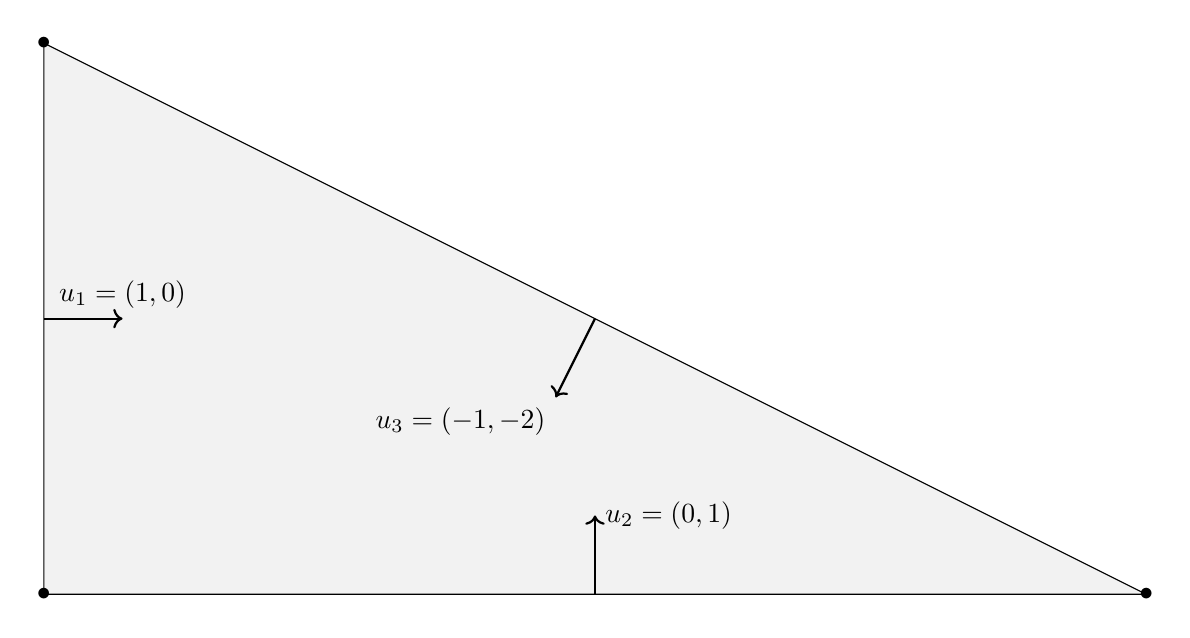
\begin{tikzpicture}
			% Polytope's outline
			\filldraw[fill=gray!10!white, draw=black] (0,0) -- (14,0) -- (0,7) -- cycle;
			\node (A) at (0,0) {$\bullet$};     
			\node (B) at (14,0) {$\bullet$};    
			\node (C) at (0,7) {$\bullet$};     
			% Circles to "zoom" into
			%        \draw (A) circle(1.25cm);
			%        \draw (B) circle(1.25cm);
			%        \draw (C) circle(1.25cm);
			% Normal vectors u_{i}
			\draw[thick, ->] (0,3.5) -- (1,3.5) node[above] {$u_{1} = (1, 0)$};
			\draw[thick, ->] (7,0) -- (7,1) node[right] {$u_{2} = (0, 1)$};
			\draw[thick, ->] (7,3.5) -- (6.5,2.5) node[below left] {$u_{3} = (-1, -2)$};
		\end{tikzpicture}
		}
	\end{figure}
\end{frame}

\begin{frame}{Toric Symplectic Orbifolds - Example}
    \begin{itemize}
        \item A vertex $v \in \Delta \subseteq \RR^{n}$ is determined by an intersection of $n$ hyperplanes, $H_{i}$:
        \[
        v = \bigcap_{i=1}^{n} \{ y \in \RR^{n}~|~\langle y, u_{i}\rangle + \lambda_{i} = 0 \} = \bigcap_{i=1}^{n} H_{i}.
        \]
        \item Moreover,
        \[
        \mu(p) = v = \bigcap_{i=1}^{n}H_{i}, \text{ for some isolated fixed-point } p.
        \]
        \item \textcolor{blue}{\underline{Def:}} Polytope $\Delta$ is called \textcolor{red}{\underline{simple}} if for each vertex $v = \bigcap_{i=1}^{n}H_{i}$, the $u_{i}$ are linearly independent.
        \item Orbifold structure group $\Gamma_{p}$ is given by
        \[
        \Gamma_{p} \cong \ZZ^{n} / \Span_{\ZZ}\{u_{i}~|~u_{i} \text{ normal vector to } H_{i} \}.
        \]
    \end{itemize}	
\end{frame}

\begin{frame}{Toric Symplectic Orbifolds - Example}
	Polytope below is the moment map image for $\CC\PP(1,2,1)$.
	\begin{figure}[h!]
		\centering
		\scalebox{0.45}{
			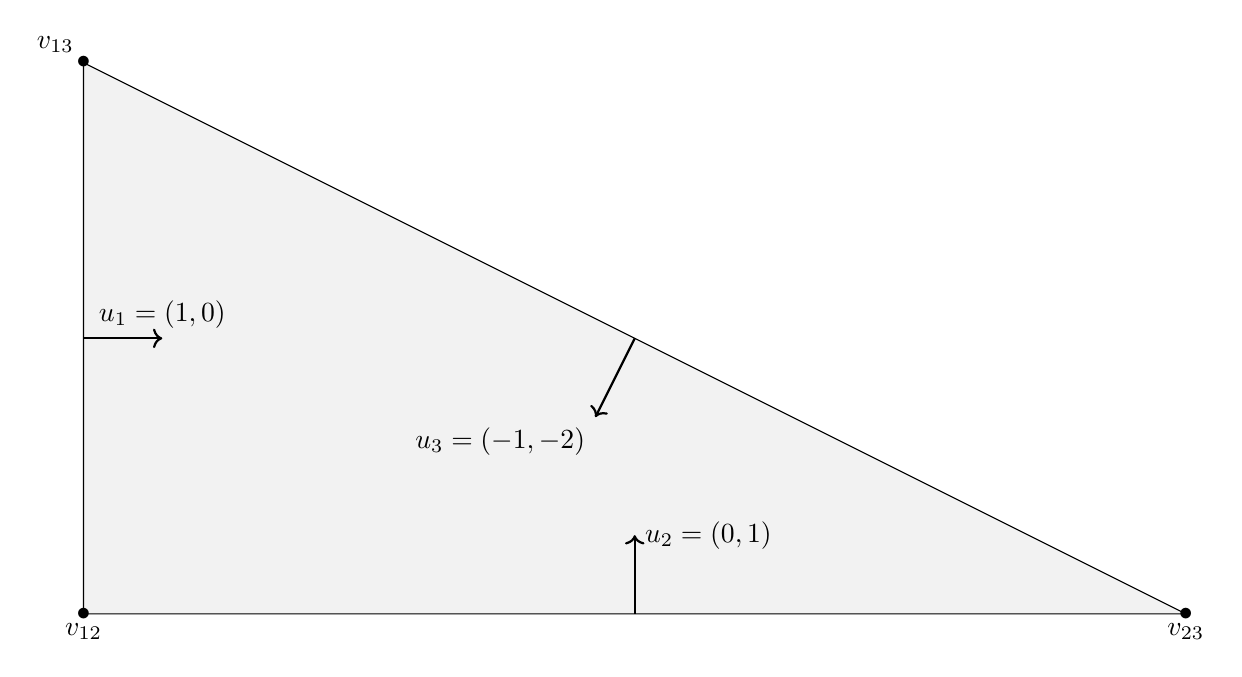
\begin{tikzpicture}
				% Polytope's outline
				\filldraw[fill=gray!10!white, draw=black] (0,0) -- (14,0) -- (0,7) -- cycle;
				\node (A) at (0,0) {$\bullet$} node[below] at (0,0) {$v_{12}$};     
				\node (B) at (14,0) {$\bullet$} node[below] at (14,0) {$v_{23}$};     
				\node (C) at (0,7) {$\bullet$} node[above left] at (0,7) {$v_{13}$};     
				% Circles to "zoom" into
				%        \draw (A) circle(1.25cm);
				%        \draw (B) circle(1.25cm);
				%        \draw (C) circle(1.25cm);
				% Normal vectors u_{i}
				\draw[thick, ->] (0,3.5) -- (1,3.5) node[above] {$u_{1} = (1, 0)$};
				\draw[thick, ->] (7,0) -- (7,1) node[right] {$u_{2} = (0, 1)$};
				\draw[thick, ->] (7,3.5) -- (6.5,2.5) node[below left] {$u_{3} = (-1, -2)$};
			\end{tikzpicture}
		}
	\end{figure}
	Top vertex $\mu(p_{13}) = v_{13}$ has:
	\[
		\Gamma_{p_{13}} \cong \ZZ^{2} / \left(u_{1}\cdot \ZZ \oplus u_{3}\cdot \ZZ \right) = \ZZ^{2} / \left(\begin{pmatrix} 1 \\ 0 \end{pmatrix} \cdot \ZZ \oplus \begin{pmatrix} -1 \\ -2 \end{pmatrix}\cdot \ZZ \right) \cong \{0\} \oplus \ZZ/2\ZZ,
	\]
	so $p_{13}$ has ``multiplicity $2$''.
\end{frame}

%------------------------------------------------
\section{Orbibundles}
%------------------------------------------------

\begin{frame}{Tangent Orbibundle}
	\begin{itemize}
		\item $(\widetilde{U}, H, \phi)$ chart for $\mathcal{X} = (X, \mathcal{U})$, action $\rho_{h} : \widetilde{U} \ra \widetilde{U}$,
		\[
		\rho_{h}(\tilde{x}) := h \cdot \tilde{x}, \qquad h \in H.  
		\]
		\item Equip tangent bundle $T\widetilde{U}$ with the $H$-action:
		\[
		h \cdot (\tilde{x}, v) := \left( h \cdot \tilde{x}, d_{\tilde{x}}\rho_{h}v \right).
		\]
		\item Get orbifold charts
		\[
		\left(T\widetilde{U}, H, q\right), \qquad q : T\widetilde{U} \ra T\widetilde{U}/H =: TU.
		\]
		\item Projection $\pi : T\widetilde{U} \ra \widetilde{U}$ is $H$-equivariant
		\[
		\implies |\pi| : TU \ra U \cong \widetilde{U}/H.
		\]
	\end{itemize}
\end{frame}

\begin{frame}{Tangent Orbibundle}
	\begin{itemize}
		\item Let $\phi(\tilde{x}) = x \in U$, and 
		\[
		|\pi|^{-1}(x) = \{ H \cdot (y,v)\ |\ y = \tilde{x} \}.
		\]
	\end{itemize}
	\textcolor{blue}{\underline{Claim:}} $|\pi|^{-1}(x) \cong T_{\tilde{x}}\widetilde{U}/\Gamma_{x} \subseteq TU$.
	\begin{itemize}
		\item
		\begin{itemize}
			\item Suppose $H \cdot (\tilde{x},v) = H \cdot (\tilde{x}, w)$
			\item $\iff$ there exists a $h \in H$ such that $h \cdot (\tilde{x},v) = (\tilde{x},w)$
			\item $\iff h \in H_{\tilde{x}}$ and $d_{\tilde{x}}\rho_{h} v = w$
			\item $\iff H_{\tilde{x}} \cdot v = H_{\tilde{x}} \cdot w$
		\end{itemize}
		\item Hence get a well-defined continuous bijection
		\[
		|\pi|^{-1}(x) \rightarrow T_{\tilde{x}}\widetilde{U}, \qquad H \cdot (\tilde{x}, v) \mapsto \Gamma_{x} \cdot v,
		\]
		with inverse the inclusion
		\[
		T_{\tilde{x}}\widetilde{U}/\Gamma_{x} \hookrightarrow TU.    
		\]
	\end{itemize}
\end{frame}

\begin{frame}{Tangent Orbibundle}
	\begin{itemize}
		\item Glue the orbifold charts $(T\widetilde{U}, H, q) \rightsquigarrow$ \textcolor{red}{\underline{tangent bundle}}, $T\mathcal{X}$, to $\mathcal{X} = (X, \mathfrak{U})$.
	\end{itemize}
	Let $\phi(\tilde{x}) = x$ for the chart $(\widetilde{U}, H, \phi)$:
	\begin{itemize}
		\item \textcolor{red}{\underline{Tangent space}} at $x$ is $T_{\tilde{x}}\widetilde{U}$ with $\Gamma_{x}$-action.
		\item \textcolor{red}{\underline{Tangent cone}} at $x$ is $C_{x}X := T_{\tilde{x}}\widetilde{U}/\Gamma_{x} \cong |\pi|^{-1}(x)$.
	\end{itemize}
\end{frame}

\begin{frame}{Sections of Orbibundles}
	\begin{itemize}
		\item Given a section $\sigma_{\widetilde{U}} : \widetilde{U} \ra T\widetilde{U}$, we get an \textcolor{red}{\underline{invariant section}} $\sigma_{U}$ by averaging,
		\[
		\sigma_{U} := \frac{1}{|\Gamma|}\sum_{\gamma \in \Gamma} \sigma_{\widetilde{U}} \circ \gamma.
		\]
		\item Similarly, if $\w$ is a differential form on $V \subset \phi(\widetilde{U})$,
		\[
		\int_{V} \w = \frac{1}{|\Gamma|}\int_{\phi^{-1}(V)} \w_{\widetilde{U}}.
		\]
		\item From $T\mathcal{X}$, get the cotangent bundle, tensor (symmetric/exterior) powers, etc., by considering each chart and gluing.
        \item Also have de Rham theory, cohomology, etc., for orbifolds.
	\end{itemize}
\end{frame}

%------------------------------------------------
\section{Index Theory}
%------------------------------------------------

\begin{frame}{Prequantisation Line Bundles}
	\begin{itemize}
		\item \textcolor{blue}{\underline{Def.:}} Let $(M, \w)$ be a compact connected $2n$-dimensional symplectic manifold. A \textcolor{red}{\underline{prequantum line bundle}} $\mcL \ra M$ is:
		\begin{itemize}
			\item A Hermitian line bundle $\mcL$;
			\item With Hermitian connection $\nabla$;
			\item Whose curvature class is $\tfrac{1}{2\pi}[\w]$;
		\end{itemize}
		\item \textcolor{blue}{\underline{Prop.:}} A prequantum line bundle $\mcL \ra M$ exists if $\tfrac{1}{2\pi}[\w] \in H^{2}(M; \ZZ)$. \\ If $M$ is simply-connected, then $\mcL$ is unique.
		\hfill \break
		\item For symplectic toric manifolds,
		\[
			\text{a quantum line bundle exists} \iff \text{its moment polytope has integral vertices.}
		\]
	\end{itemize}
\end{frame}

\begin{frame}{Hirzeburch-Riemann-Roch Formula}
	\begin{block}{Theorem (Hirzebruch-Riemann-Roch)}
		Let $(M, \w)$ be a symplectic manifold, and $\mcL \ra M$ a prequantum line bundle. Then
		\[
			\dim H^{0}(M; \mcL) = \int_{M} e^{c_{1}(\mcL)} \wedge \Td_{M}(TM),
		\]
		where $e^{c_{1}(\mcL)}$ and $\Td_{M}(TM)$ are the Chern character and Todd class for $M$, respectively.
	\end{block}
	Assuming $TM$ splits by the splitting principle as $TM \cong \bigoplus_{i=1}^{n} V_{i}$, the Todd class is given by
	\[
		\Td_{M}(TM) = \prod_{i=1}^{n} \frac{c_{1}(V_{i})}{1 - e^{-c_{1}(V_{i})}}.
	\]
\end{frame}

\begin{frame}{Hirzeburch-Riemann-Roch Formula - Example}
	\begin{itemize}
		\item Let $M = \CC\PP^{2}$, $\mcL = \mc{O}(k)$;
		\item Then $c_{1}(\mc{O}(k)) = kH$, where $\langle H \rangle = H^{2}(\CC\PP^{2}; \ZZ)$;
		\item Total chern class for $T\CC\PP^{2}$:
		\[
			c(T\CC\PP^{2}) = (1 + H)^{3} = 1 + 3H + 3H^{2} = c_{0} + c_{1} + c_{2} \implies c_{1} = 3H,~c_{2} = 3H^{2}.
		\]
		\item Gives Todd class: $\Td_{\CC\PP^{2}}(T\CC\PP^{2}) = 1 + \frac{c_{1}}{2} + \frac{c_{1}^{2} + c_{2}}{12} = 1 + \frac{3}{2}H + H^{2};$
		\item HRR thus gives:
		\begin{align*}
				\dim H^{0}(\CC\PP^{2}; \mc{O}(k)) &= \int_{\CC\PP^{2}}e^{c_{1}(\mc{O}(k))} \wedge \Td_{\CC\PP^{2}}(T\CC\PP^{2}) \\ &= \int_{\CC\PP^{2}}\left( 1 + kH + (k^{2}/2)H^{2} \right) \wedge \left(1 + (3/2)H + H^{2}\right) \\ &= \int_{\CC\PP^{2}} \left(1 + 3k/2 + (k^{2}/2)\right)H^{2} + \ldots = \frac{(k+1)(k+2)}{2}.
		\end{align*}
	\end{itemize}
\end{frame}

\begin{frame}{Equivariant Localisation}
	If $M$ has a $T$-action, we can generalise the HRR theorem to an \textcolor{red}{\underline{equivariant character}} $\chi : T \ra \mathcal{R}(T)$ (representation ring for $T$).
	\begin{block}{Theorem (Atiyah-Bott, Berline-Vergne)}
		Let $(M, \w, T^{n}, \mu)$ be a symplectic toric manifold, and $\mcL \ra M$ a prequantum line bundle. Let $M^{T}$ denoted the fixed-point set for the $T^{n}$-action. For $t \in T$, let $\xi \in \mft$ be such that $e^{\xi} = t$.
		\hfill \break
		Then
		\[
			\chi(e^{\xi}) = \sum_{p \in M^{T}} \frac{e^{\langle \mu(p),~\xi\rangle}}{\prod_{i = 1}^{n}\left(1 - e^{\langle \alpha_{i,p},~ \xi \rangle }\right)},
		\]
		where $\alpha_{i,p}$ are the isotropy weights for the $T^{n}$-representation, $T_{p}M$.
	\end{block}
\end{frame}

\begin{frame}{Equivariant Localisation for Symplectic Toric Manifolds}
	For $(M, \w, T^{n}, \mu)$ a symplectic toric manifold, the isotropy data can be read off from the moment polytope, $\Delta = \mu(M)$:
	\begin{itemize}
		\item For $p \in M^{T}$, its image is a vertex $v = \mu(p)$ of $\Delta$;
		\item The isotropy weights $\alpha_{i,p}$ point along the edges from $v$.
	\end{itemize}
	Example for $(\CC\PP^{2}, k\w, T^{2}, \mu)$:
	\begin{figure}[h!]
		\centering
		\scalebox{0.45}{
			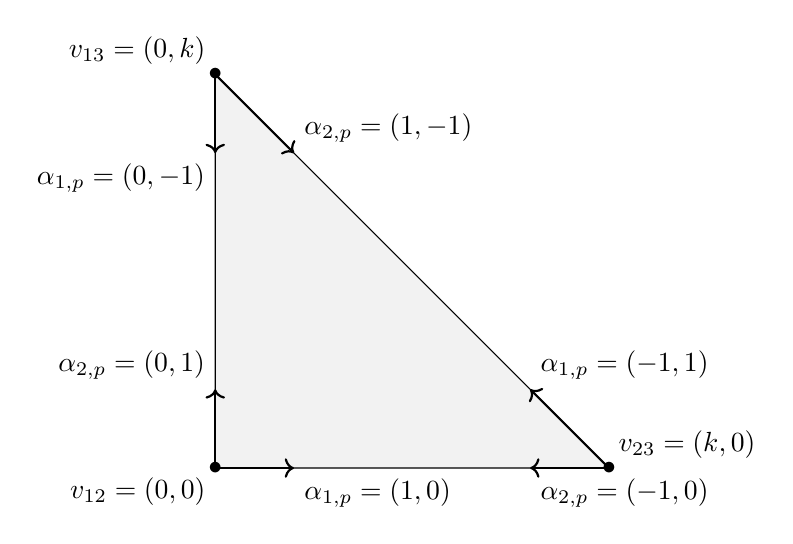
\begin{tikzpicture}
				% Polytope's outline
				\filldraw[fill=gray!10!white, draw=black] (0,0) -- (5,0) -- (0,5) -- cycle;
				\node (A) at (0,0) {$\bullet$} node[below left] at (0,0) {$v_{12} = (0,0)$};     
				\node (B) at (5,0) {$\bullet$} node[above right] at (5,0) {$v_{23} = (k,0)$};     
				\node (C) at (0,5) {$\bullet$} node[above left] at (0,5) {$v_{13} = (0,k)$};     
				% Edge vectors \alpha_{i,p}
				\draw[thick, ->] (0,0) -- (1,0) node[below right] {$\alpha_{1,p} = (1, 0)$};
				\draw[thick, ->] (0,0) -- (0,1) node[above left] {$\alpha_{2,p} = (0, 1)$};
				\draw[thick, ->] (5,0) -- (4,1) node[above right] {$\alpha_{1,p} = (-1, 1)$};
				\draw[thick, ->] (5,0) -- (4,0) node[below right] {$\alpha_{2,p} = (-1,0)$};
				\draw[thick, ->] (0,5) -- (0,4) node[below left] {$\alpha_{1,p} = (0, -1)$};
				\draw[thick, ->] (0,5) -- (1,4) node[above right] {$\alpha_{2,p} = (1,-1)$};
			\end{tikzpicture}
		}
	\end{figure}
\end{frame}

\begin{frame}{$(\CC\PP^{2}, k\w, T^{2}, \mu)$ Example}
	\begin{figure}[h!]
		\centering
		\scalebox{0.45}{
			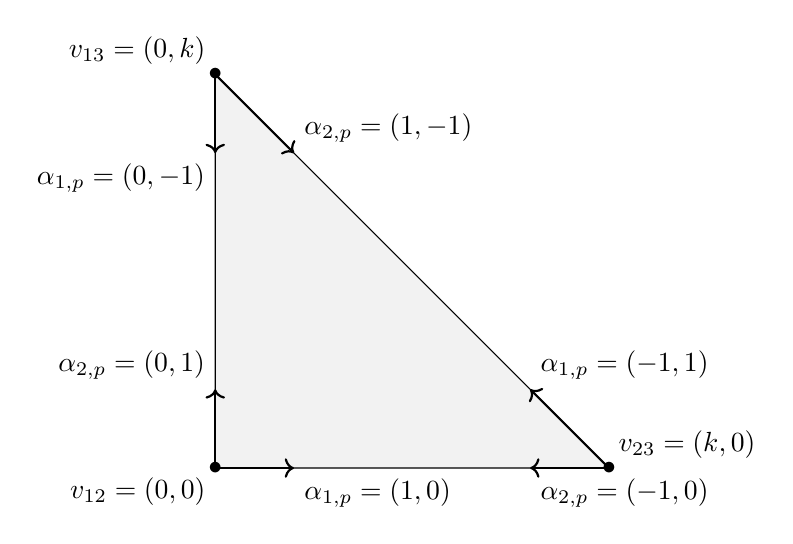
\begin{tikzpicture}
				% Polytope's outline
				\filldraw[fill=gray!10!white, draw=black] (0,0) -- (5,0) -- (0,5) -- cycle;
				\node (A) at (0,0) {$\bullet$} node[below left] at (0,0) {$v_{12} = (0,0)$};     
				\node (B) at (5,0) {$\bullet$} node[above right] at (5,0) {$v_{23} = (k,0)$};     
				\node (C) at (0,5) {$\bullet$} node[above left] at (0,5) {$v_{13} = (0,k)$};     
				% Edge vectors \alpha_{i,p}
				\draw[thick, ->] (0,0) -- (1,0) node[below right] {$\alpha_{1,p} = (1, 0)$};
				\draw[thick, ->] (0,0) -- (0,1) node[above left] {$\alpha_{2,p} = (0, 1)$};
				\draw[thick, ->] (5,0) -- (4,1) node[above right] {$\alpha_{1,p} = (-1, 1)$};
				\draw[thick, ->] (5,0) -- (4,0) node[below right] {$\alpha_{2,p} = (-1,0)$};
				\draw[thick, ->] (0,5) -- (0,4) node[below left] {$\alpha_{1,p} = (0, -1)$};
				\draw[thick, ->] (0,5) -- (1,4) node[above right] {$\alpha_{2,p} = (1,-1)$};
			\end{tikzpicture}
		}
	\end{figure}
	For $(x,y) \in T^{2}$:
	\begin{align*}
		\chi(x,y) &= \frac{1}{(1-x)(1-y)} + \frac{x^{k}}{(1- x^{-1})(1- x^{-1}y)} + \frac{y^{k}}{(1 - y^{-1})(1 - xy^{-1})} \\ &= (1 + x + x^{2} + \ldots + x^{k}) + y(1 + x + x^{2} + \ldots + x^{k-1}) + \ldots + y^{k} \\ &=  \sum_{k_{1} + k_{2} \leq k} x^{k_{1}}y^{k_{2}} \overset{(x,y) \ra (1,1)}{\longrightarrow} \sum_{k_{1} + k_{2} \leq k} 1 = \frac{(k+1)(k+2)}{2} = \dim H^{0}(\CC\PP^{2}; \mc{O}(k)).
	\end{align*}
\end{frame}

\begin{frame}{$(\CC\PP^{2}, k\w, T^{2}, \mu)$ Example}
	Letting $(x,y) \ra (1,1)$, we get that
	\[
		\chi(1,1) = \dim H^{0}(\CC\PP^{2}; \mc{O}(k)).
	\]
	Calculate
	\begin{align*}
		\chi(x,y) = \sum_{k_{1} + k_{2} \leq k} x^{k_{1}}y^{k_{2}} \longrightarrow \sum_{k_{1} + k_{2} \leq k} 1 = \frac{(k+1)(k+2)}{2} = \dim H^{0}(\CC\PP^{2}; \mc{O}(k)).
	\end{align*}
	Moreover, $T^{2}$ acts on $\CC\PP^{2}$ as: $[z_{1}:z_{2}:z_{3}] \mapsto [xz_{1}:yz_{2}:z_{3}]$,
	\[
		x^{k_{1}}y^{k_{2}} \leftrightsquigarrow z_{1}^{k_{1}}z_{2}^{k_{2}}z_{3}^{k-k_{1}-k_{2}}.
	\]
\end{frame}

\begin{frame}{... Orbifolds?}
		\begin{block}{Theorem (Kawasaki-Riemann-Roch)}
			Let $(M, \w, T^{n}, \mu)$ be a symplectic toric orbifold, and $\mcL \ra M$ a prequantum line bundle. Let $M^{T}$ denoted the fixed-point set for the $T^{n}$-action. For $t \in T$, let $\xi \in \mft$ and $e^{\xi} = t$.
			\hfill \break
			Then
			\[
			\chi(e^{\xi}) = \sum_{p \in M^{T}} \left( \frac{1}{|\Gamma_{p}|} \sum_{\gamma \in \Gamma_{p}} \frac{e^{\langle \mu(p),~\xi\rangle}}{\prod_{i = 1}^{n}\left(1 - e^{2\pi \sqrt{-1}\langle \alpha_{i,p},\gamma\rangle}e^{\langle \alpha_{i,p},\xi \rangle }\right)} \right),
			\]
			where $\alpha_{i,p}$ are isotropy weights, and $\Gamma_{p}$ is the orbifold structure group for $p \in M^{T}$.
		\end{block}
	When $\Gamma_{p} = \{0\}$ for each $p$, we recover the equivariant HHR formula.
\end{frame}

\begin{frame}{$\CC\PP(1,2,1)$ Example}
	\begin{figure}[h!]
		\centering
		\scalebox{0.5}{
			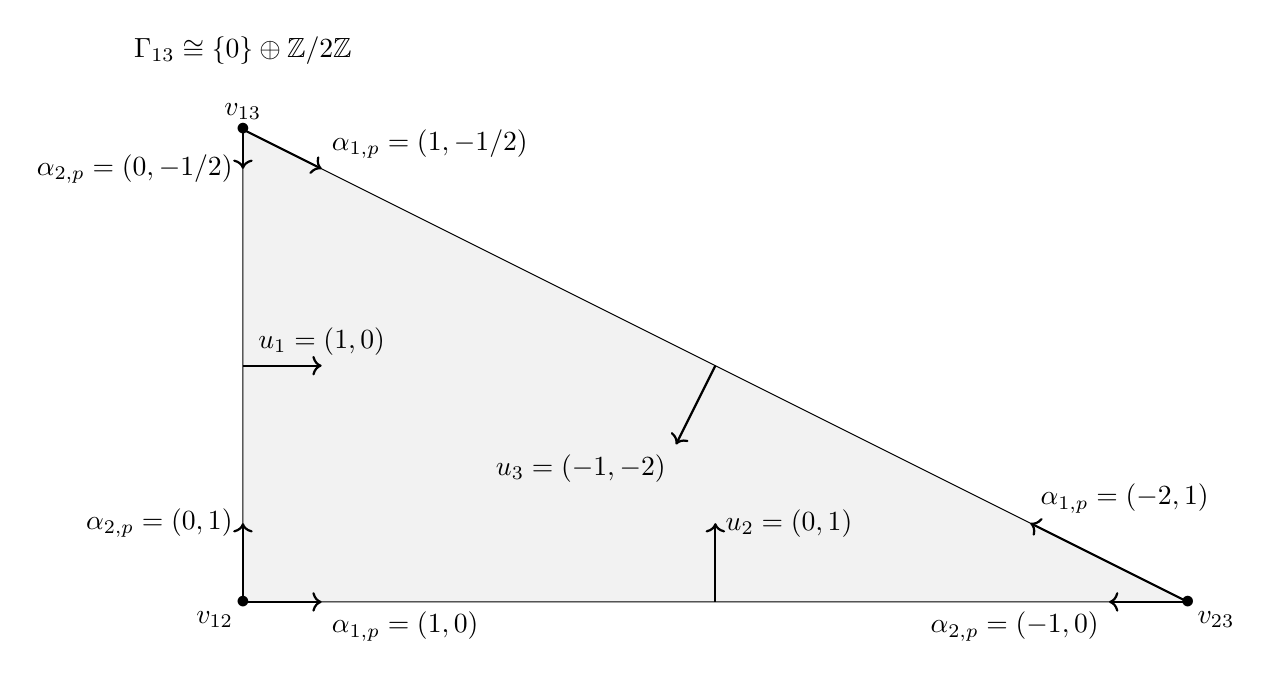
\begin{tikzpicture}
				% Polytope's outline
				\filldraw[fill=gray!10!white, draw=black] (0,0) -- (12,0) -- (0,6) -- cycle;
				\node (A) at (0,0) {$\bullet$} node[below left] at (0,0) {$v_{12}$};
				\node (B) at (12,0) {$\bullet$} node[below right] at (12,0) {$v_{23}$};
				\node (C) at (0,6) {$\bullet$} node[above] at (0,6) {$v_{13}$};
				\node at (0,7) {$\Gamma_{13} \cong \{0\} \oplus \ZZ/2\ZZ$};
				% Normal vectors u_{i}
				\draw[thick, ->] (0,3) -- (1,3) node[above] {$u_{1} = (1, 0)$};
				\draw[thick, ->] (6,0) -- (6,1) node[right] {$u_{2} = (0, 1)$};
				\draw[thick, ->] (6,3) -- (5.5,2) node[below left] {$u_{3} = (-1, -2)$};
				% Isotropy weights \alpha_{i,p}
				\draw[thick, ->] (0,0) -- (1,0) node[below right] {$\alpha_{1,p} = (1, 0)$};
				\draw[thick, ->] (0,0) -- (0,1) node[left] {$\alpha_{2,p} = (0, 1)$};
				\draw[thick, ->] (12,0) -- (10,1) node[above right] {$\alpha_{1,p} = (-2, 1)$};
				\draw[thick, ->] (12,0) -- (11,0) node[below left] {$\alpha_{2,p} = (-1, 0)$};
				\draw[thick, ->] (0,6) -- (1,5.5) node[above right] {$\alpha_{1,p} = (1, -1/2)$};
				\draw[thick, ->] (0,6) -- (0,5.5) node[left] {$\alpha_{2,p} = (0, -1/2)$};
			\end{tikzpicture}
		}
	\end{figure}
	Contribution from $p_{13}$:
	\begin{align*}
		&\frac{1}{2}\left( \frac{y^{k}}{(1 - xy^{-1/2})(1 - y^{-1/2})} + \frac{y^{k}}{(1 - e^{\pi\sqrt{-1}}xy^{-1/2})(1 - e^{\pi\sqrt{-1}}y^{-1/2})} \right) \\ &= \frac{y^{k}}{2}\left( \frac{1}{(1 - xy^{-1/2})(1 - y^{-1/2})} + \frac{1}{(1 + xy^{-1/2})(1 + y^{-1/2})} \right)
	\end{align*}
\end{frame}

\begin{frame}{$\CC\PP(1,2,1)$ Example}
    With the other two smooth points:
    \begin{align*}
        \chi(x,y) &= \frac{y^{k}}{2}\left( \frac{1}{(1 - xy^{-1/2})(1 - y^{-1/2})} + \frac{1}{(1 + xy^{-1/2})(1 + y^{-1/2})} \right) \\
        &+ \frac{1}{(1-x)(1-y)} + \frac{x^{2k}}{(1-x^{-1})(1 - x^{-2}y) } \\
        &= \sum_{k_{1} + 2k_{2} \leq 2k} x^{k_{1}}y^{k_{2}} \longrightarrow \chi(1,1) = k^{2} + 2k + 1.
    \end{align*}
    We find that
    \[
        \dim H^{0}(\CC\PP(1,2,1) ; \mc{O}(2k)) = k^{2} + 2k + 1,
    \]
    corresponding to the basis of monomials
    \[
        (x,y) \cdot [z_{1}, z_{2}, z_{3}] = [xz_{1} : y^{2}z_{2}:z_{3}]  \leftrightsquigarrow z_{1}^{k_{1}}z_{2}^{k_{2}}z_{3}^{2k - k_{1} - 2k_{2}}
    \]
\end{frame}

%----------------------------------------------------------------------------------------

\end{document}